
%\documentclass[12pt]{report}

\documentclass[12pt]{article}
%\usepackage{natbib}  % used for citations
\usepackage[parfill]{parskip} %used for formatting style of text



\usepackage{graphicx,fancyhdr}
\usepackage{amssymb,amsmath}
\usepackage{epigraph,fancyvrb,eqparbox}
\usepackage[multiple]{footmisc}
\usepackage{menukeys}
\usepackage{menukeys}
\usepackage{url}
\usepackage[colorlinks = true, linkcolor = blue, urlcolor = blue]{hyperref}
\usepackage{setspace}

\pagestyle{fancyplain}

%\usepackage{hyperref}
%\usepackage{epsf,psfig,graphicx,fancyheadings}
% \textwidth 7in
% \textheight 9in
% \oddsidemargin 0in
% \topmargin -.25in

%-----------------------------------------------
% The following settings are from Dr. Davidian's
% ST810A Handout on Advanced LaTeX Features

%\setlength{\paperheight}{11.0in}
%\setlength{\paperwidth}{8.5in}

%%%%%%%%%%%%%%%%%%%%%%%%%%%%%%%%%%%%%%%%%%%%%%%%%
% For Desktop @ CalPoly (for Postscript)

%\setlength{\oddsidemargin}{0.5in}
%\setlength{\evensidemargin}{0.5in}
%\setlength{\topmargin}{-.5in}

%%%%%%%%%%%%%%%%%%%%%%%%%%%%%%%%%%%%%%%%%%%%%%%%%
% For Laptop @ Calpoly (for Postscript)

% \setlength{\oddsidemargin}{0.in}
% \setlength{\evensidemargin}{0.in}
% \setlength{\topmargin}{0.25in}

%%%%%%%%%%%%%%%%%%%%%%%%%%%%%%%%%%%%%%%%%%%%%%%%%
% For Desktop @ CalPoly (for PDF)

%\setlength{\oddsidemargin}{0.in}
%\setlength{\evensidemargin}{0.in}
%\setlength{\topmargin}{-.5in}
%
%%%%%%%%%%%%%%%%%%%%%%%%%%%%%%%%%%%%%%%%%%%%%%%%%%
%% For Laptop @ Calpoly (for PDF)
%
%% \setlength{\oddsidemargin}{0.in}
%% \setlength{\evensidemargin}{0.in}
%% \setlength{\topmargin}{0.25in}
%
%
%
%\setlength{\oddsidemargin}{0.0in}
%\setlength{\topmargin}{-0.5in}
%\setlength{\headheight}{0.20in}
%\setlength{\headsep}{3ex}
%\setlength{\baselineskip}{2ex}
%\setlength{\textheight}{9in}
%\setlength{\textwidth}{6.4in}
%\renewcommand{\baselinestretch}{1.1}

% Sets margins to 1 in
\addtolength{\oddsidemargin}{-.5in}%
\addtolength{\evensidemargin}{-.5in}%
\addtolength{\textwidth}{1in}%
\addtolength{\textheight}{1.3in}%
\addtolength{\topmargin}{-.8in}%

%\setlength{\headheight}{0.20in}
%\setlength{\headsep}{3ex}
%\setlength{\headrulewidth}{0.2pt}
%\setlength{\footrulewidth}{0.15pt}
%\setlength{\parskip}{2.3ex}
% %set to no indentation
%\setlength{\parindent}{0.0in}
%\setlength{\baselineskip}{2ex}
%\setlength{\textheight}{9.in}
%\setlength{\textwidth}{6.5in}

\def \doublespace{\openup 2\jot}
% For double or 1.5 spacing
%\renewcommand{\baselinestretch}{1.5}
\tolerance=500

\def\boxit#1{\vbox{\hrule\hbox{\vrule\kern6pt
\vbox{\kern6pt#1\kern6pt}\kern6pt\vrule}\hrule}}
\renewcommand{\theequation}{\thesection.\arabic{equation}}
% The following for TOC
%\renewcommand{\thepage}{\roman{page}}
% to be followed by this for the main text
\renewcommand{\thepage}{\arabic{page}}


%-----------------------------------------------

%%%%%%%%%%%%%%%%%%%%%%%%%%%%%%%%%%%%%%
%Define any shortcut aliases below

\newtheorem{theo}{Theorem}[section]

\newenvironment{note}{\begin{quote}\emph{Note:\ }}{\end{quote}}
\newenvironment{defn}{
\begin{description}
\item[Definition ]}
{\end{description}}

\newenvironment{ttscript}[1]{%
    \begin{list}{}{%
    \settowidth{\labelwidth}{\texttt{#1}}
    \setlength{\leftmargin}{\labelwidth}
    \addtolength{\leftmargin}{\labelsep}
    \setlength{\parsep}{0.5ex plus0.2ex minus0.2ex}
    \setlength{\itemsep}{0.3ex}
    \renewcommand{\makelabel}[1]{\texttt{##1\hfill}}}}
    {\end{list}}

\newcommand{\bt}{\begin{tabular}}
\newcommand{\et}{\end{tabular}}
\newcommand{\bc}{\begin{center}}
\newcommand{\ec}{\end{center}}
\newcommand{\bi}{\begin{itemize}}
\newcommand{\ei}{\end{itemize}}
\newcommand{\be}{\begin{enumerate}}
\newcommand{\ee}{\end{enumerate}}
\newcommand{\bq}{\begin{quote}}
\newcommand{\eq}{\end{quote}}
\newcommand{\vect}[1]{\mbox{\boldmath $ #1$}}
\newcommand{\avg}[1]{$\overline{#1}$}
\newcommand{\bmp}{\begin{minipage}}
\newcommand{\emp}{\end{minipage}}
\newcommand{\hr}{\u{\hspace{7in}}}
\newcommand{\sr}{\u{\hspace{5in}}}
\newcommand{\chs}{\chi^2}

\newcommand{\labn}[1]{\Large{\textbf{\fbox{Lab #1}}}\hspace{0.1in} \normalsize{\emph{Some of these problems may be more challenging than others. Please feel free to work with others, attend office hours, or post on the course discussion forum if you need help.  While collaboration with other students is encouraged, each student is responsible for submitting his or her own work.  This assignment should be submitted in one well-commented SAS program.  For any questions that require a written answer, do so in the SAS comments.  Be sure to re-name the uploaded SAS scripts according to the naming convention}} \texttt{LastnameFirstinitial\textunderscore Lab\#.sas} (\emph{e.g.,} \texttt{PileggiS\textunderscore Lab#1.sas}).}


\newcommand{\hd}[1]{\lhead{STAT 330/530: Lab #1}\rhead{Pileggi, FA17}}
\newcommand{\bs}{\underline{\hspace{0.5in}}}

%\newcommand{\bv}{\footnotesize
%\bmp{.5\textwidth}
%\begin{Verbatim}[frame=single,label=SAS Code,commandchars=\\\{\}],xrightmargin=.5\textwidth}
%
%\newcommand{\ev}{\end{Verbatim}
%\emp
%\normalsize}

\newcommand{\bv}{\begin{code}}
\newcommand{\ev}{\end{code}}

 \newenvironment{code}[1]%
  {\vspace{.1in}\footnotesize\Verbatim[frame=single,label=SAS Code,commandchars=\\\{\},xrightmargin=#1\textwidth,framesep=.2in,labelposition=all]}
  {\endVerbatim\normalsize}

\newenvironment{craw}[2]%
{\vspace{.1in}\footnotesize\Verbatim[frame=single,label=#2,commandchars=\\\{\},xrightmargin=#1\textwidth,framesep=.2in,labelposition=all]}
  {\endVerbatim\normalsize}

\newenvironment{cbox}[1]%
{\vspace{.1in}\footnotesize\Verbatim[frame=single,commandchars=\\\{\},xrightmargin=#1\textwidth,framesep=.2in,labelposition=all]}
  {\endVerbatim\normalsize}

\newcommand{\head}[1]{\large \textbf{#1} \normalsize}

\newcommand{\ttt}[1]{\textbf{\texttt{#1}}}


\newcommand{\bsval}[1]{\underline{\hspace{0.2in}{[#1]}\hspace{0.2in}}}

\newcommand{\ttb}{\textbf}
\newcommand{\tte}{\emph}
\newcommand{\ttu}{\underline}



\newcommand{\jdhr}{\vspace{0.2in}\hrule}


\newcommand{\uspace}[1]{\underline{\hspace{#1}}}

\newenvironment{ident}{\begin{list}{}{}
         \item[]}{\end{list}}

\newenvironment{proposition}{
\begin{description}
\item[Proposition: ]}
{\end{description}}

\newcommand{\bpr}{\begin{proposition}}
\newcommand{\epr}{\end{proposition}}



% \newenvironment{example}
%     {
%         \begin{list}{\textbf{Example:}}
%         {
%         \settowidth{\labelwidth}{}
%         \setlength{\leftmargin}{\labelwidth}
%         }
%     }
%     {\end{list}}


\newenvironment{example}{
\jdhr \vspace{-.17in}\jdhr
\textbf{Example: }}
{}

\newcommand{\bex}{\begin{example}}
\newcommand{\eex}{\end{example}}

\newenvironment{onyourown}{
\jdhr \vspace{-.17in}\jdhr
\textbf{On Your Own: }}
{}

\newcommand{\boy}{\begin{onyourown}}
\newcommand{\eoy}{\end{onyourown}}


%\newenvironment{debug}{
%\jdhr \vspace{-.17in}\jdhr
%\ttb{Debug the Code}
%\fbox{
%\bmp{.95in}
%\includegraphics[height=.35in]{C:/images/bug4.jpg}\includegraphics[height=.35in]{C:/images/buggy8.jpg}
%\emp}
%}
%{\jdhr}

\newenvironment{debug}{
\jdhr \vspace{-.17in}\jdhr
\ttb{Debug the Code: }
\fbox{
\bmp{.95in}
\includegraphics[height=.35in]{C:/images/bug4.jpg}\includegraphics[height=.35in]{C:/images/mushi90.jpg}
\emp}
}
{}


\newcommand{\bbug}{\begin{debug}}
\newcommand{\ebug}{\end{debug}}


\begingroup
  \catcode `_=11
  \gdef\myuscore{_}
  \catcode `~=11
  \gdef\mytilde{~}
  \catcode `\|=0
  \catcode `\\=11
  |gdef|mybs{\}
|endgroup

%Define any shortcut aliases above


%....................................................................
%....................................................................
%....................................................................
%....................................................................
%....................................................................
%....................................................................
%....................................................................
%....................................................................



\usepackage{amssymb}
				

\begin{document}
\hd{18}
\labn{18}
\vskip10pt \noindent \textbf{Notes: (1) For this lab you do not need to do any statistical tests or interpret any p-values - I am only asking for descriptive statistics.  (2) You will need to research different kinds of SAS informats to complete this lab. (3) You are not allowed to modify the raw data files!}
\begin{enumerate}
\item Store the computer location of your data sets as a macro variable.
\item In 1983 New York city presented evidence in court that Brink's (a collections contractor) employees had been stealing parking meter money - delivering to the city less than the total collections. The data consists of the amount of money collected each month by Brink’s and a control sample that was taken by the city.
\item[]
\begin{tabular}{l}
\ttt{Data\_parking.dat} \\
\hline
Date \\
\$ collected by state of NY\\
\$ collected by city of NY  \\
Brink’s (1) or other contractor (0) \\
\end{tabular}
\begin{enumerate}
\item Read the data into a temporary data set in SAS, using the macro variable you created in (1).
\item Use a SAS procedure to verify that all variables are numeric (including date).
\item Visually check that your date read in correctly by verifying that the first observation has a SAS date value of 6330. (No SAS code/comment required.)
\item In one PROC, calculate the average amount of money collected by the city of NY among Brink's contractors and among other contractors.  Note the averages in a comment in your SAS code and identify which is higher.
\end{enumerate}
%\item
%The following data file contains information about a music collection.
%\item[]
%\begin{tabular}{l}
%\ttt{Data\_music\_files.dat} \\
%\hline
%Album name (A1, A2, etc.)\\
%Song title \\
%Size of file in bytes
%\end{tabular}
%\begin{enumerate}
%\item Read the data into a temporary data set in SAS, using the macro variable you created in (1). \emph{Note: you can include the .mp3 in the song title variable.}
%\item Create a variable in the data set the represents the length of the song title (ie, the number of characters in the song title).  \emph{Hint: look up character functions.}
%\item In one PROC, determine if the relationship between title length and bytes is linear and estimate the correlation between these two variables. Discuss these results in a comment in your SAS code.  \emph{Hint: you need to examine one piece of output to determine if the relationship is linear and a \underline{separate} piece of output to determine the correlation.}
%\item You probably noticed an unusual observation in your scatterplot.  Use a PROC to identify the name of the song that corresponds to this observation, and note this in a comment in your SAS code.
%\end{enumerate}
\item  We have information on some earthquakes from December 2010 and January 2011.
\item[]
\begin{tabular}{l}
\ttt{Earthquake.dat}\\
\hline
Map name \\
Magnitude \\
Date and time \\
Latitude \\
Longitude \\
Depth \\
Location \\
\end{tabular}
\begin{enumerate}
\item Read the data into a temporary data set in SAS, using the macro variable you created in (1). \emph{Hint:  In SAS, dates and times can be read into one variable - a date/time variable.}
\item Use a SAS procedure to verify that only map name and location are character variables - all other variables (including date and time) should be numeric.
\item Use the \ttt{series} statement in \ttt{PROC SGPLOT} to re-create the figure below exactly, which shows a time series of the magnitude of the earthquakes.
\item[] 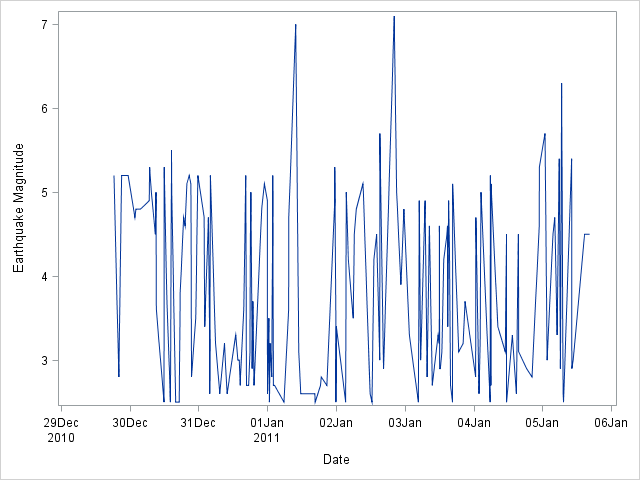
\includegraphics[width=0.55\textwidth]{earthquakets.png}
\item Recall that the \ttt{where} statement in SAS can use additional operators compared to the \ttt{if} statement (Lecture 6).  Using a \ttt{PROC} with a \ttt{where} statement, identify how many earthquakes occurred in (1) Mexico, and (2) Alaska.  (This can be two separate PROCs, one for each location.)  State your findings in a comment in your SAS code.
%\item Did more earthquakes occur in the Northern or Southern hemisphere?
%\item Earthquakes with magnitude of 5 or more are considered moderate or worse. How many of our earthquakes fall into this group?
\end{enumerate}
\item The Rose Bowl is a college tradition that dates back to the early 1900's.
\item[]
\underline{\ttt{rosebowl.dat}}
\item[]  Game date, \fbox{\ttt{c}} Team 1, Team 1 score, \fbox{\ttt{c}} Team 2, Team 2 score
\item[] \emph{Note: the two variables with the} \fbox{\ttt{c}} \emph{symbol should be read in as character variables.}
\begin{enumerate}
\item Open the \ttt{rosebowl.dat} in a text editor such as notepad.  Describe the features that you see in the data that you will need to address when reading it in to SAS.  Note your findings as a comment in your SAS code.
\item Read the data into SAS using the macro variable you created in question (1).
\item Use a SAS procedure to verify that your variables read in correctly as character or numeric.
\item Create a new variable that indicates the following possible game outcomes: ``team 1 wins'', ``team 2 wins'', and ``tie''.
\item Use a SAS procedure to print the games which resulted in a tie.  Apply a format to the game date variable so that it displays as a calendar date rather than a SAS date value.
\item Use any PROCs and/or DATA steps necessary to create a variable that represents the cumulative total number of games won by team 1.  Do not include ties in this cumulative sum.
\item Create a data set which only has one observation per team 1 and that only keeps the variables team 1 name and cumulative total number of wins.  Print this data set.  So that you may check your work, the first three observations are displayed below.
\item[]
\begin{craw}{.0}{first 3 observations}
  Obs    team1                    num_wins
    1    Alabama                      4
    2    Arizona State                1
    3    California                   2
 \end{craw}
\end{enumerate}
\item Ben \& Jerry's is a popular ice cream manufacturer that was founded in 1978.
\item[] \underline{\ttt{BenAndJerrys.dat}}
\item[]  \fbox{\ttt{c}} flavor name, portion size (g), calories, calories from fat, fat (g), saturated fat (g), trans fat (g), cholesterol (mg), sodium (mg), total carbohydrate (g), \fbox{\ttt{c}} dietary fiber (g), sugars (g), protein (g), \fbox{\ttt{c}} year introduced, \fbox{\ttt{c}} year retired, \fbox{\ttt{c}} content description, \fbox{\ttt{c}} notes
\item[] \emph{Note: the six variables with the} \fbox{\ttt{c}} \emph{symbol should be read in as character variables.}
\begin{enumerate}
\item Open the \ttt{BenAndJerrys.dat} in a text editor such as notepad.  Describe the features that you see in the data that you will need to address when reading it in to SAS.  Note your findings as a comment in your SAS code.
\item Read the data into SAS using the macro variable you created in question (1).  Use the \ttt{INFILE} statement
\item[]\fbox{\ttt{INFILE "\&path.BenAndJerrys.dat" DLM="," DSD ;}}
\item[] which contains options discussed in the extra material (not required) of Lecture 18.
\item Use a SAS procedure to verify that your variables read in correctly as character or numeric.
\item Subset the data to keep only flavors that that can be purchased at the grocery store.  A flavor that is ``Scoop Shop Exclusive'' can only be purchased in the Ben \& Jerry's ice cream store; otherwise, the flavor can be purchased at the grocery store.
\item Recreate the following plot.  Your axis labels do not need to be displayed exactly as seen below (the figure below just uses the variable names for axis labels).
\item[] 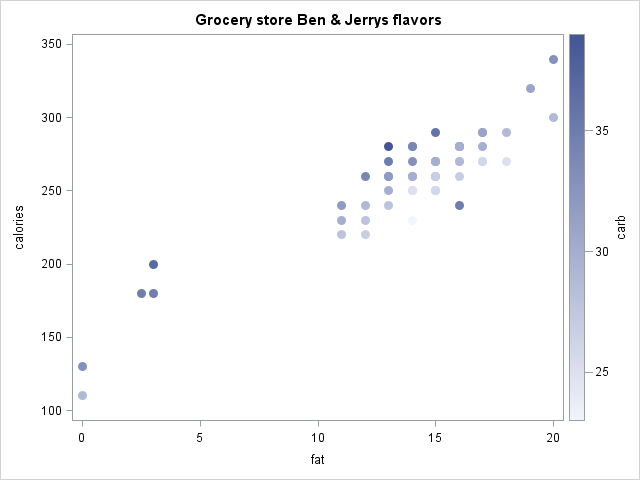
\includegraphics[width=0.75\textwidth]{BenJerryscatter.png}
\end{enumerate}

\end{enumerate}
\end{document} 